\documentclass[tikz,border=5pt]{standalone}
\usepackage[UTF8]{ctex}\usepackage{amsmath,amssymb}
\usetikzlibrary{arrows.meta,calc}
\definecolor{ink}{HTML}{243447}\definecolor{blue}{HTML}{2765A2}
\definecolor{green}{HTML}{3F7D5B}\definecolor{red}{HTML}{B74739}
\tikzset{body/.style={draw=ink,thick},vec/.style={draw=blue,thick,-{Latex}},guide/.style={gray!65,dashed},dim/.style={ink,{Latex}-{Latex}},line cap=round,line join=round}
\begin{document}
\begin{tikzpicture}[x={(1cm,0)},y={(.42cm,.22cm)},z={(0,1cm)}]
 \filldraw[body,fill=gray!12](0,0,0)--(4,0,0)--(4,0,1.35)--(0,0,1.35)--cycle;
 \filldraw[body,fill=gray!18](4,0,0)--(4,2,0)--(4,2,1.35)--(4,0,1.35)--cycle;
 \filldraw[body,fill=blue!8](0,0,1.35)--(4,0,1.35)--(4,0,2)--(0,0,2)--cycle;
 \filldraw[body,fill=blue!12](4,0,1.35)--(4,2,1.35)--(4,2,2)--(4,0,2)--cycle;
 \filldraw[body,fill=blue!4](0,0,2)--(4,0,2)--(4,2,2)--(0,2,2)--cycle;
 \draw[guide](0,2,1.35)--(4,2,1.35);
 \node at(2,0,1.68){$n_1=1.52$};\node at(2,0,.6){$n_2=1.72$};
 \node[right]at(3,2,3){$n_0=1$};
 \draw[blue,thick](1,1,2)--(1,1,4);
 \draw[vec](1,1,4)--(1,1,3.3)node[midway,left]{入射};
 \draw[green,thick,-{Latex}](1,1,2.2)--(1,1,3.05)node[midway,right]{反射};
 \draw[dim](-.4,0,1.35)--(-.4,0,2)node[midway,left]{$h$};
\end{tikzpicture}
\begin{tikzpicture}
 \fill[blue!6](-.4,1)rectangle(6.4,2.6);
 \draw[body](-.4,2.6)--(6.4,2.6)(-.4,1)--(6.4,1);
 \node[left]at(-.4,3.3){$n_0$};\node[left]at(-.4,1.8){$n_1$};\node[left]at(-.4,.5){$n_2$};
 \draw[blue,thick](1.1,2.6)--(1.1,4);
 \draw[vec](1.1,4)--(1.1,3.4);\draw[green,thick,-{Latex}](1.1,2.7)--(1.1,3.25);
 \node[above]at(1.1,4){直接反射};\node at(1.1,.3){$a$};
 \draw[blue,thick](4.3,1)--(4.3,4);
 \draw[vec](4.3,4)--(4.3,3.4);\draw[vec](4.3,2.5)--(4.3,2.05);
 \draw[green,thick,-{Latex}](4.3,1.15)--(4.3,1.8);\draw[green,thick,-{Latex}](4.3,2.75)--(4.3,3.25);
 \node[above]at(4.3,4){一次膜内反射};
 \node at(4.3,.3){$(1-a^2)b e^{i\delta}$};
 \draw[dim](6.8,1)--(6.8,2.6)node[midway,right]{$h$};
 \node at(3,-.5){传播历史分栏，实际反射束重合};
\end{tikzpicture}
\begin{tikzpicture}
 \node[draw=blue,rounded corners,fill=blue!4,minimum width=2.6cm,minimum height=1.15cm](E0)at(0,0){$E_0=(1-a^2)b e^{i\delta}$};
 \node[draw=blue,rounded corners,fill=blue!4,minimum width=2cm,minimum height=1.15cm](E1)at(4.3,0){$E_1=E_0q$};
 \node[draw=blue,rounded corners,fill=blue!4,minimum width=2cm,minimum height=1.15cm](E2)at(7.8,0){$E_2=E_0q^2$};
 \draw[vec](E0)--(E1)node[midway,above=8mm]{多一次往返};
 \draw[vec](E1)--(E2)node[midway,above=8mm]{再往返};
 \draw[vec](E2)--(9.5,0)node[right]{$\cdots$};
 \node at(4,-1.3){$q=r_{10}r_{12}e^{i\delta}=-ab e^{i\delta}$};
\end{tikzpicture}
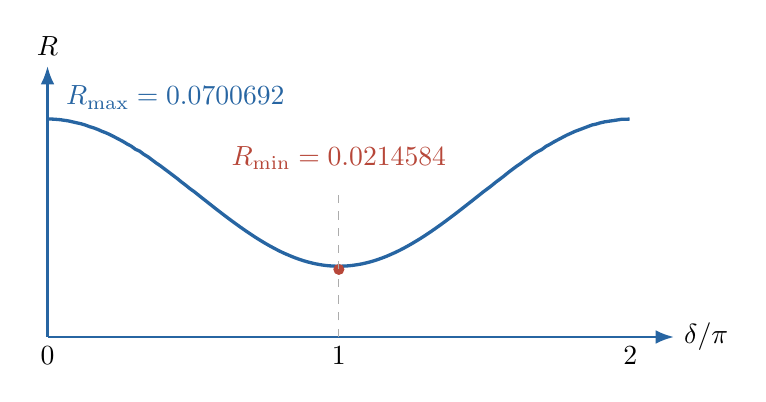
\begin{tikzpicture}[x=3.7cm,y=40cm]
 \draw[vec](0,0)--(2.15,0)node[right]{$\delta/\pi$};
 \draw[vec](0,0)--(0,.086)node[above]{$R$};
 \draw[blue,very thick,domain=0:2,samples=140]
 plot(\x,{(.04257999496+.003810394757+2*sqrt(.04257999496*.003810394757)*cos(180*\x))/(1+.04257999496*.003810394757+2*sqrt(.04257999496*.003810394757)*cos(180*\x))});
 \draw[guide](1,0)--(1,.02145835359);\fill[red](1,.02145835359)circle(2pt);
 \draw[guide](1,.02145835359)--(1,.047);
 \node[red,above]at(1,.05){$R_{\min}=0.0214584$};
 \node[blue,right]at(.03,.076){$R_{\max}=0.0700692$};
 \foreach\x in{0,1,2}{\node[below]at(\x,0){$\x$};}
\end{tikzpicture}
\end{document}
